\documentclass[times, 10pt,twocolumn]{article} 

\usepackage{geometry}
\usepackage{graphicx}
\usepackage{amssymb}
\usepackage{subfigure}
\usepackage{cite}
\usepackage{hyphenat}
\usepackage{latex8}
\usepackage{times}

\newbox\subfigbox % Create a box to hold the subfigure. 
\makeatletter 
\newenvironment{subfloat}% % Create the new environment. 
{\def\caption##1{\gdef\subcapsave{\relax##1}}% 
\let\subcapsave=\@empty % Save the subcaption text. 
\let\sf@oldlabel=\label 
\def\label##1{\xdef\sublabsave{\noexpand\label{##1}}}% 
\let\sublabsave\relax % Save the label key. 
\setbox\subfigbox\hbox 
\bgroup}% % Open the box... 
{\egroup % ... close the box and call \subfigure. 
\let\label=\sf@oldlabel 
\subfigure[\subcapsave]{\box\subfigbox}}% 
\makeatother 

\title{FlatCAD and FlatLang: Kits by Code} 

\author{
Gabe Johnson\\
Carnegie Mellon University
}

\begin{document}

\maketitle

\begin{abstract}
The \nohyphens{FlatCAD} system lets you create physical construction
kits by coding in the LOGO-like \nohyphens{FlatLang}
language. Designers often use structured CAD tools to specify physical
form. Programming offers an alternative and powerful method for
designing shapes. This paper describes our experimental
domain-specific language used to program and manufacture physical
shape in the domain of construction kits.
\end{abstract}

\section{Introduction}

A LEGO kit consists of plastic pieces that snap together
vertically. ``Hub and strut'' kits such as Tinker Toys feature rigid
links that fit in holes in hubs. Most kits contain pieces that vary in
size, length, or the way they fit together. Despite---or perhaps
because of---kit simplicity, they support people in building creative,
complex assemblies.

Instead of building from parts we are given we could design new kits,
enabling us to work in different ways. To explore this we developed
\nohyphens{FlatCAD}, a system supporting users to develop novel
construction kits manufactured with laser cutters.

\nohyphens{FlatCAD} targets fabrication of physical objects using flat
material such as wood, acrylic, or paper. The material may be
\underline{f}olded, \underline{l}ayered, \underline{a}ttached, and
\underline{t}rimmed in various ways to make physical
constructions---hence ``flat'' CAD. \nohyphens{FlatCAD} models are
made by programming in a LOGO-like language called
\nohyphens{FlatLang}. Figure~\ref{fig:physical-output} shows examples
of kits created with \nohyphens{FlatCAD}.

\begin{figure}[h]
   \centering
     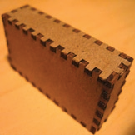
\includegraphics[width=0.9in]{physical-output-boxcad-correct.pdf}
   \hspace{2mm}
     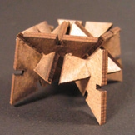
\includegraphics[width=0.9in]{physical-output-jessica-correct.pdf}
   \hspace{2mm}
     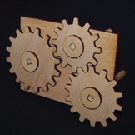
\includegraphics[width=0.9in]{physical-output-gears-correct.pdf}
   \caption{Physical output of \nohyphens{FlatCAD}: parametric boxes, polygon construction kit, mechanical gears.}
   \label{fig:physical-output}
\end{figure}

\subsection{A Mechanical Construction Kit}

\begin{figure}[h]
\centering
  \begin{subfloat}
    \begin{minipage}{2.6in} 
      \footnotesize
\begin{verbatim}
coaxial(gear(10), piston_wheel())
link(4).draw()
\end{verbatim}
    \end{minipage}% 
  \end{subfloat} 
  \begin{minipage}{1.3in}
      \centering 
    \begin{subfloat}
      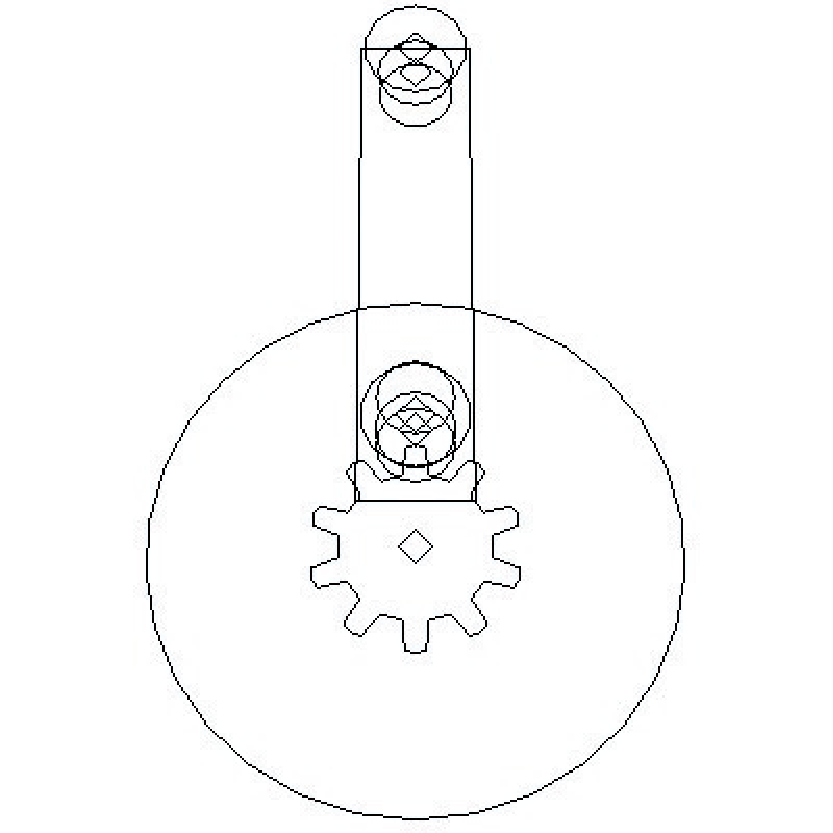
\includegraphics[width=1.3in]{mechanism-graphics-correct.pdf}
    \end{subfloat}
  \end{minipage}
  \begin{minipage}{1.3in}
      \centering 
    \begin{subfloat}
      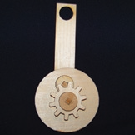
\includegraphics[width=1.3in]{mechanism-physical-correct.pdf}
    \end{subfloat}
  \end{minipage}
  \caption{High-level \nohyphens{FlatLang} code, graphics, and
    physical output for a simple mechanism.}
  \label{fig:machine-code} 
\end{figure} 

Physical mechanical construction kits may come with a few kinds of
parts, but FlatLang lets us program any type of part we like. This
lets us make constructions using parts tailored to our particular
needs. Say our goal is to make a toy vehicle with a puppet `driving'
it. We want the puppet to move horizontally as the vehicle rolls. To
do this we convert the wheel's radial motion to linear motion that
moves the puppet.

One way of converting angular to linear motion is by using a piston
wheel (Figure~\ref{fig:machine-code}). It has an off-center axle
attached to a rigid strut. When the other end of the strut is
constrained to move along a straight path, rotating the wheel causes
the strut to move back and forth linearly.

We can parameterize our automaton. Changing the wheel's radius changes
the puppet's up-and-down frequency. Adding gears changes the puppet's
speed in relation to the forward motion of the vehicle. Lengthening
the distance between the piston wheel center and its off-center axle
will make the puppet move a greater distance. The complete program for
this automaton is shown in Figure~\ref{fig:automaton-parameteric}.

\begin{figure}[h]
  \begin{subfloat}
    \begin{minipage}{2.6in}
      \footnotesize
\begin{verbatim}
define parametric_automaton
  (g1_n_teeth, g2_n_teeth, offset)

  wheel_1 = wheel()
  wheel_2 = wheel()
  gear_1 = gear(g1_n_teeth)
  gear_2 = gear(g2_n_teeth)
  piston = piston_wheel(offset)
  piston.strut = link()

  coaxial(wheel_1, mesh(gear_1, 
          coaxial(gear_2, piston_wheel)), 
          wheel_2)
done
\end{verbatim}
    \end{minipage}
  \end{subfloat}
  \caption{A parametric version of the toy vehicle automaton.}
  \label{fig:automaton-parameteric}
\end{figure}

\subsection{Why Not Use Illustrator?}

One might ask, ``If your goal is to make toys on a laser cutter, why
not use Illustrator?''  The answer is that algorithmic generation of
form can be expressive in ways that direct manipulation is not. While
other tools are based on direct manipulation, in \nohyphens{FlatCAD}
the primary interaction mode is coding. From a human designer's
perspective, there may be significant advantages for using one
interaction mode over another. This area deserves further
exploration.

\section{Related Work}

The LOGO language provides a ``microworld'' to explore programming
\cite{papert-mindstorms}. LOGO graphics are based on two-dimensional
``turtle geometry'' \cite{abelson-turtle-geometry}. Drawings are made
by programming an on-screen ``turtle'' to move or turn. A recent
LOGO-like language called FormWriter used a ``flying turtle'' that
operated in 3D \cite{gross-formwriter}. In addition to drawing lines,
FormWriter had primitive drawing functions for creating 3D objects
such as cones, cylinders, and boxes.

Several recent systems have been developed to explore software
supporting rapid prototyping and construction kits. For example,
Triskit pieces are wafer-like sheets of acrylic. Their edges attach
with finger joints \cite{martin-triskit}. Triskit pieces are
`programmed' by providing dimensions to a Java applet and then
`printed' using a rapid prototyping machine. The Furniture Factory and
the Designosaur capture freehand sketches used to generate dollhouse
furniture and wooden dinosaur skeletons \cite{oh-fab}. Mori and
Igarashi's Plushie system let people design plush toys that can then
be printed and sewn \cite{mori-plushie}.

The MachineShop enables users to design mechanical systems such as toy
automata, made from parts like gears and cams
\cite{blauvelt-automata}. Rather than directly editing the parameters
or shape of such components, MachineShop users indicate behavioral
qualities such as the distance a cam follower moves as the cam
rotates. It then generates the part that provides the desired
behavior.

Commercial design systems lets users specify exact dimensions and
angles using mouse and keyboard commands. But models can also be
specified with code instructions. \nohyphens{SolidWorks} lets
designers establish constraints such as ``X is halfway between A and
B''. Regardless of how A or B change, the system ensures X is between
them. Modeling systems such as Maya or SketchUp provide scripting
capabilities so users can write programs to directly generate or
modify models.

\section{\nohyphens{FlatLang} Programming}

\nohyphens{FlatLang} is a dynamically typed, interpreted language. The
interpreter is written in Java, and FlatLang code is parsed with ANTLR
\cite{parr-antlr}. Its syntax resembles Python's, though indentation
is not significant.

Figure~\ref{fig:pentahedron} shows a simple \nohyphens{FlatLang}
program for making a pentahedron. In this example, the
\textnhtt{dihedralAngle} is declared and initialized to
125$^\circ$. Next, the code declares two
functions. \textnhtt{triangle} produces an equilateral triangle of
parametric size. The \textnhtt{goNext} routine `rolls' and positions
the turtle for the next operation. The final function loops four
times, explicitly creating four of the five faces of our square
pyramid. The fifth face (the base of the pyramid) is created
implicitly from the turtle's path.

\begin{figure}
  \centering 
  \begin{subfloat}% 
    \begin{minipage}{1.8in} 
      \footnotesize
\begin{verbatim}
dihedralAngle = 125

define triangle(size)
  repeat(3)
    forward(size)
    left(120)
  done
done

define goNext(size)
  roll(-dihedralAngle)
  forward(size)
  right(90)
  roll(dihedralAngle)
done

define pentahedron()
  roll(dihedralAngle)
  repeat(4)
    triangle(3)
    goNext(3)
  done
done
\end{verbatim}

    \end{minipage}% 
  \end{subfloat} 
  \begin{minipage}{1.0in}
    \begin{subfloat}
      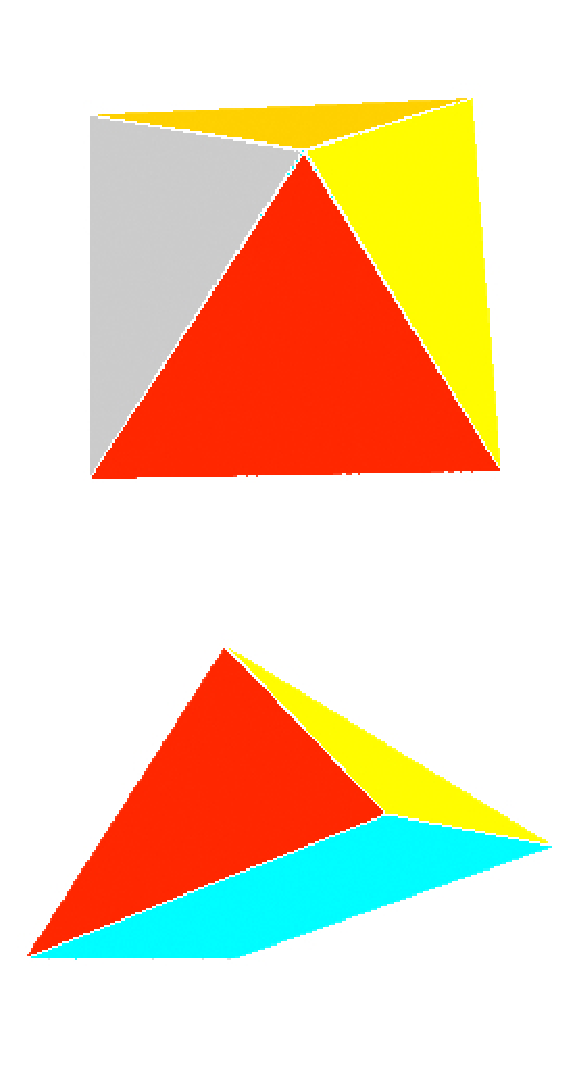
\includegraphics[width=1.0in]{pentahedron.pdf}
    \end{subfloat}
  \end{minipage}
  \caption{Low-level \nohyphens{FlatLang} and graphics for a
    pentahedron.}
    \label{fig:pentahedron}
\end{figure} 

Construction kits are powerful because of the piece's regular,
predictable shapes and the ways they attach. To this end we support
programming above the level of turtle geometry. We have developed a
library of parametric mechanical parts such as gears, piston wheels
and n-bar linkages. We have also developed ways to express how the
parts fit together. Others can use our library or develop their
own. For example we may write \textnhtt{coaxial(gear(12),~gear(24))}
to make two gears sharing an axis. One gear has twelve teeth, the
other has twice that number.

The on-screen representation shows how parts relate---the gear and
piston wheel's centers are at the same location in
Figure~\ref{fig:machine-code}. However, when this is sent to a laser
cutter, those parts must be separated and arranged to make efficient
use of material. \nohyphens{FlatLang's} \textnhtt{part} command
creates logical collections of geometry to be kept together when
printing. Each `part' represents a piece in the construction kit. This
lets the programmer focus on creating systems of parts without
manually separating them on the screen.

\subsection{Turtle Tree}

\nohyphens{FlatCAD} records the turtle's activity in a data structure
called the \textit{Turtle Tree}. Tree nodes are turtle operations, of
which there are three kinds: geometry, pen, and naming commands.
Geometry commands modify the turtle's position or heading
(e.g. \textnhtt{forward}, \textnhtt{left}, \textnhtt{roll}). Pen
commands (\textnhtt{up}, \textnhtt{down}) toggle the turtle's visual
trail. Geometry and pen nodes may have at most one child.

\subsubsection{Named turtle nodes}

Named nodes are created with the \textnhtt{mark(s)} function. They may
have any number of children. Figure~\ref{fig:centered_polygon}
demonstrates the \textnhtt{mark} command.

A FlatLang function may create arbitrarily complex geometry. Turtle
Trees let us `rewind' to geometric features without needing to know
the details of the function that created it. The programmer only need
know the names of points of interest. 

The \textnhtt{backto(s)} command sets the current insertion location
to a previously named position
\textnhtt{s}. Figure~\ref{fig:turtle-tree} depicts a Turtle Tree after
using the \tetnhtt{backto} command. Turtle operations inherit the
location, direction, and pen state of its parent.

\subsubsection{Shapes}

Procedures that generate a shape typically begin and end at the same
locations. However, we may want to draw a shape beginning from one
particular location. Turtle commands executed in a \textnhtt{shape}
block are not added to the turtle tree, but to a separate circular
structure. Because this structure is circular, we may draw shapes
beginning from arbitrary nodes using the \textnhtt{draw} and
\textnhtt{from} commands. Shapes are illustrated in
Figure~\ref{fig:shapes}.

\begin{figure}[h]

  \begin{minipage}{}
    \begin{subfloat}
      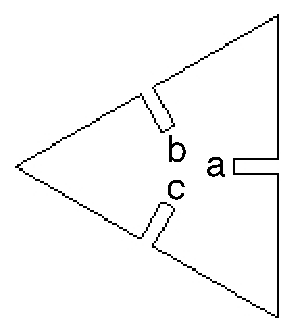
\includegraphics[width=1.0in]{notched_triangle.pdf}
      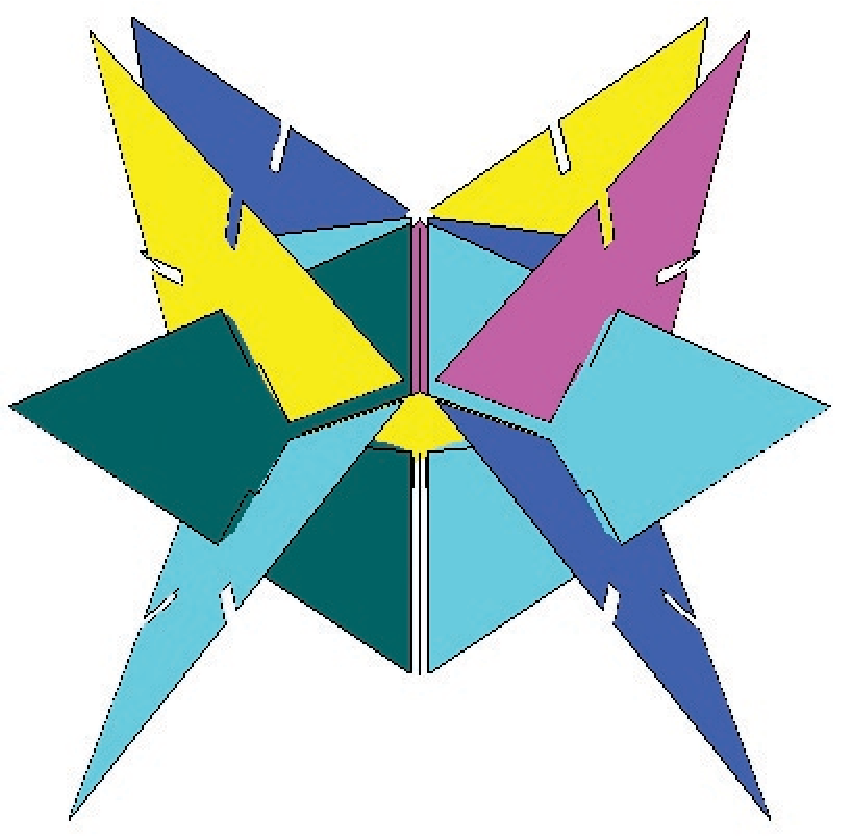
\includegraphics[width=1.0in]{shapes-complete.pdf}
    \end{subfloat}
  \end{minipage}

  \begin{subfloat}
    \begin{minipage}{2.6in}
      \footnotesize
\begin{verbatim}
define notched_tri(len, dep, wid)
  angle = 360 / 3
  notch(len, dep, wid, "a")
  left(angle)
  notch(len, dep, wid, "b")
  left(angle)
  notch(len, dep, wid, "c")
  left(angle)
done

define go(s, ttl)
  draw(s, "a")
  from("b","c")
    pitch(90)
    left(180)
    if (ttl > 0)
      go(s, ttl - 1)
    done
  done
done

shape("tri")
  notched_tri(3, 0.4, 0.1)
done

go("tri", 3)
\end{verbatim}
    \end{minipage}
  \end{subfloat}
  \caption{Recursive \nohyphens{FlatLang} code demonstrating shape
    definition and drawing.}
  \label{fig:shapes}
\end{figure}

\begin{figure*}
  \begin{subfloat}
    \begin{minipage}{1.6in}
      \footnotesize
\begin{verbatim}
notch(3, 0.5, 0.2, "X")
backto("X")
left(10)
notch(3, 0.5, 0.2, "Y")
\end{verbatim}
    \end{minipage}
  \end{subfloat}
  \begin{subfloat}
    \begin{minipage}{5.0in}
      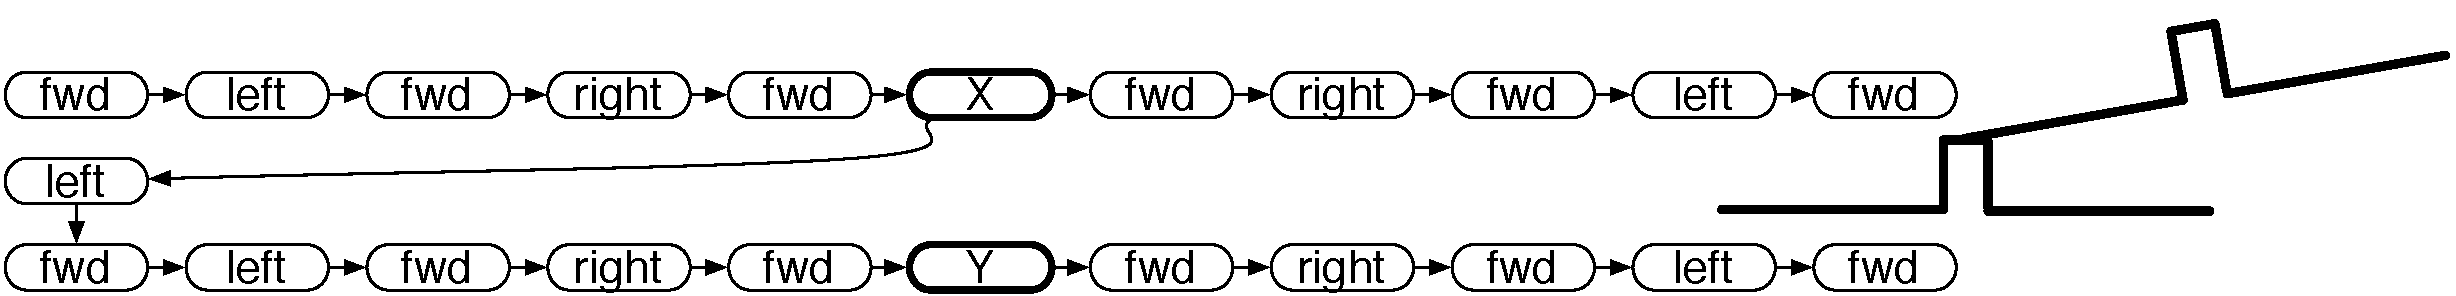
\includegraphics[width=5.0in]{turtle_tree_graph.pdf}
      \end{minipage}
  \end{subfloat}
  \caption{Code, associated Turtle Tree, and graphic output illustrating \textnhtt{backto}.}
  \label{fig:turtle-tree}
\end{figure*}

\subsubsection{Absolute geometric commands}

Most geometric turtle commands indicate change \textit{relative} to
the turtle position. FlatLang also supports \textit{absolute}
geometric commands. The \textnhtt{pos} and \textnhtt{dir} commands
supply the absolute turtle position and directions. Programs may use
previously stored positions or direction with the \textnhtt{drawto}
and \textnhtt{facedir} commands. Absolute geometry is useful when we
need to connect points but we are not able (or do not want) to
calculate turtle geometry between points.

\begin{figure}[h]
  \begin{subfloat}
    \begin{minipage}{2.6in}
      \footnotesize
\begin{verbatim}
define centered_polygon(sides, radius)
  angle = 360 / sides
  points = [] ; initialize empty list
  up()
  mark("middle")
  i = 0
  repeat(sides+1)
    backto("middle")
    left(i * angle)
    forward(radius)
    points = cons(pos(), points)
    i = i+1
  done
  down()
  repeat(points.n)
    p = first(points)
    points = rest(points)
    drawto(p)
  done
  backto("middle")
done
\end{verbatim}
    \end{minipage}
  \end{subfloat}
  \caption{\nohyphens{FlatLang} showing absolute and differential
    geometry and \textnhtt{mark} and \textnhtt{backto}.}
  \label{fig:centered_polygon}
\end{figure}

Figure~\ref{fig:centered_polygon} illustrates
\textnhtt{mark}/\textnhtt{backto} and
\textnhtt{pos}/\textnhtt{drawto}. After lifting the pen it marks the
``middle''. Next, vertices are calculated by rotating the turtle
and moving forward. The first point is stored twice
in order to complete the tour. Next the pen is lowered and points
connected by repeated calls to \textnhtt{drawto}. This code makes
equilateral polygons exactly centered at the initial position.

\section{Discussion and Future Work}

While programming is a powerful method to express some ideas, it is by
no means a panacea. Currently, the only mode of interacting with
FlatCAD is to program in FlatLang. We envision alternate modes of
interaction for FlatCAD, making it more ``equal opportunity''
\cite{cockburn-leogo} by letting users choose the right mode for the
task. Programming is good at some tasks and poor at others. When it is
inappropriate, the benefits of other expressive modes (e.g. sketching
or direct manipulation) could be used.

Unlike other LOGO implementations, \nohyphers{FlatCAD} analyzes the
turtle's path and (for example) provides visual feedback when the
turtle has completed a polygon. Further, the turtle tree is a
manipulable record of the turtle's history, and can be used to insert
named locations, record, play back, or edit sequences of turtle
operations.

Frequently, errors are discovered only as the parts are physically
assembled. If the program had an awareness of the desired behavior it
could provide critical feedback before users invest time in
fabricating a physical model.

It is also possible to generate models based on functional
descriptions, as in MachineShop \cite{blauvelt-automata}. High level
descriptions such as ``translate radial motion into harmonic linear
motion'' could be translated into code.

\section{Conclusion}

We have introduced \nohyphens{FlatCAD}, a design tool for programming
and manufacturing physical shape. FlatLang lets us program individual
parts or build complete assemblies by writing code specifying how
parts fit together. We may then produce models using a laser
cutter. The process of designing mechanisms with code can be powerful.

\section{Acknowledgments}

This work was funded by NSF Grant ITR-0326054. I am grateful to Mark
Gross, Ellen Do, and Yeonjoo Oh for advice and support on this
project.

\bibliographystyle{latex8}
\bibliography{sketch-bibliography}

\end{document}  
